%%%%%%%%%%%%%%%%%%	
\section{Balanced Search Tree} (\S 18.1, page 488) A B-tree $T$ is a rooted tree (whose root is $T.root$) having the following properties.  
	\begin{enumerate}
		\item Every node $x$ has the following attributes.
		\begin{enumerate}
			\item $x.n$, the number of keys currently stored in node $x$, 
			\item The $x.n$ keys themselves, $x.key_1, x.key_2, \dots, x.key_{x.n}$, stored in nondecreasing order, so that $x.key_1 \le x.key_2 \le \cdots \le x.key_{x.n}$.
			\item $x.leaf$, a boolean value that is \verb|True| if $x$ is a leaf and \verb|False| if $x$ is an internal node.  
		\end{enumerate}
		\item Each internal node $x$ also contains $x.n+1$ pointers, $x.c_1, x.c_2, \dots, x.c_{x.n+1}$ to its children.  Leaf nodes have no children, and so their $c_i$ attributes are undefined.  
		\item The keys $x.key_i$ separate the ranges of keys stored in each subtree.  If $k_i$ is any key stored in the subtree with root $x.c_i$, then 
		$$k_1 \le x.key_1 \le k_2 \le x.key_2 \le \cdots \le x.key_{x.n} \le k_{x.n+1}$$
		\item All leaves have the same depth, which is the tree's height, $h$.  
		\item Nodes have lower and upper bounds on the number of keys they can contain.  We express these bounds in terms of a fixed integer $t \ge 2$ called the {\it minimum degree} of the B-tree.  
		\begin{enumerate}
			\item Every node other than the root must have at least $t-1$ keys.  Every internal node other than the root thus has at least $t$ children.  If the tree is nonempty, the root must have a least one key.  
			\item Every node may contain at most $2t-1$ keys.  Therefore, an internal node may have at most $2t$ children.  We say that a node is {\it full} if it contains exactly $2t-1$ keys.  
		\end{enumerate}
	\end{enumerate} 
	\index{Balanced Search Tree!Definition!\S 18.0 - 18.3}
	
\subsection{Method for Inserting and Deleting a Key}

In a B-tree (Balanced binary tree) with minimum degree $t$, each node other than the root must have at least $t-1$ keys, and each node including the root must have at most $2t-1$ keys.  When we delete or insert a key, we don't know up front the node from which we're going to insert or delete the key, and we want to make just one pass from root to leaf, so we're going to adjust appropriately as we go.  

When deleting a key, when passing from the root to a leaf, if a node and its children together can be merged (contain no more than $2k-1$ keys), merge them.

When inserting a key, when passing from the root to a leaf, if a node has the maximum ($2k-1$) number of keys, split it.  
	
%%%%%%%%%%
\subsection{Old Exam Questions}

Note:  Why do they introduce keys with subscripts, instead of just using $A$ through $Z$?  Twenty-six keys is plenty for these exercises.  

%%%%%
\subsubsection{S19 \#L1}
	
	 Given a B-tree with the minimum degree of $t=3$ below, show the results after (i) deleting $B$, (ii) followed by inserting $M$, (iii) then followed by deleting $T$, and then inserting $M_t$ for $M<M_t<N$
	
	\index{Balanced Search Tree!S19 \#L1}
	
\
	
\hfil	\begin{tikzpicture}[x=12mm, y=15mm]
		\node [rectangle, draw, fill=gray] (0) at (0,0) {$P$};
		\node [rectangle, draw, fill=gray] (1) at (-3,-1) {$C G$};
		\node [rectangle, draw, fill=gray] (2) at (3,-1) {$T X$};
		\node [rectangle, draw, fill=gray] (3) at (-5,-2) {$A B$};
		\node [rectangle, draw, fill=white] (4) at (-3,-2) {$D E$};
		\node [rectangle, draw, fill=gray] (5) at (-1,-2) {$JKL NO$};
		\node [rectangle, draw, fill=gray] (6) at (1,-2) {$QRS$};
		\node [rectangle, draw, fill=gray] (7) at (3,-2) {$UV$};
		\node [rectangle, draw, fill=gray] (8) at (5,-2) {$YZ$};
		\draw [-triangle 60] (0) -- (1); 
		\draw [-triangle 60] (0) -- (2); 
		\draw [-triangle 60] (1) -- (3); 
		\draw [-triangle 60] (1) -- (4); 
		\draw [-triangle 60] (1) -- (5); 
		\draw [-triangle 60] (2) -- (6); 
		\draw [-triangle 60] (2) -- (7); 
		\draw [-triangle 60] (2) -- (8); 
	\end{tikzpicture}
	
	Note:  The different shading of the nodes is not relevant.  They copied this from some book exercise where the node color indicated some step in a process that is not described here.  
	
\subsubsection{Solution}

{\bf Original Tree}

\
	
\hfil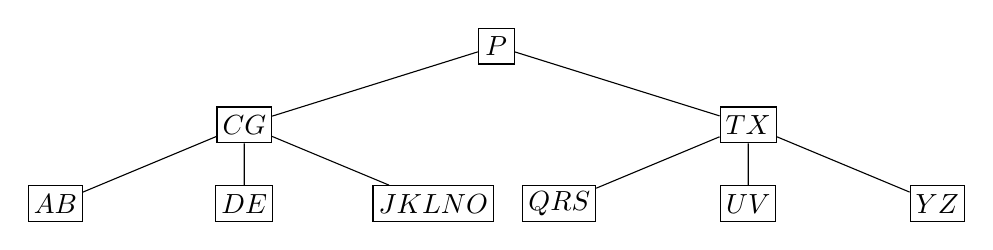
\begin{tikzpicture}[
	level 1/.style={level distance=10mm,sibling distance=64mm},
	level 2/.style={level distance=10mm,sibling distance=24mm},
	level 3/.style={level distance=10mm,sibling distance=16mm},
	inner sep=2pt,every node/.style={draw,rectangle,minimum size=3ex}]
  \node {$P$}
  child {node {$CG$}
  	child {node {$AB$}}
	child {node {$DE$}}
	child {node {$JKLNO$}}
  }
  child {node {$TX$}
  	child {node {$QRS$}}
	child {node {$UV$}}
	child {node {$YZ$}}
  };
\end{tikzpicture}

\

{\bf i. Delete $B$.}

Instructions on ``Deleteing a key from a B-tree,'' part 3.  Starting at $x = root$, ``If the key $k$ is not present in internal node $x$, determine the root $x.c_i$ of the appropriate subtree that must contain $k$, if $k$ is in the tree at all.''  Since $B<P$, we must go to the left to $x.c_1 = CG$.    

``If $x.c_i$ has only $t-1$ keys, execute step 3a or 3b as necessary to guarantee that we descend to a node containing at least $t$ keys.  Then finish by recursing on the appropriate child of $x$.  

It is true that $x.c_1 = CG$ has only $t-1=2$ keys.  

``3a.  If $x.c_i$ has only $t-1$ keys but has an immediate sibling with at least $t$ keys,....''  Not true, since the only sibling of $CG$ is $TX$, which also has only $2<t$ keys.  

``3b.  If  $x.c_i$ and both of $x.c_i$'s immediate siblings have $t-1$ keys, merge $x.c_i$ with one sibling, which involves moving a key from $x$ down into the new merged node to become the median key for that node.''

We need to merge $CG$ and $TX$, moving $P$ down into the new merged node to become the median key for that node.  



  First merge $P$, $CG$, and $TX$.  

\
	
\hfil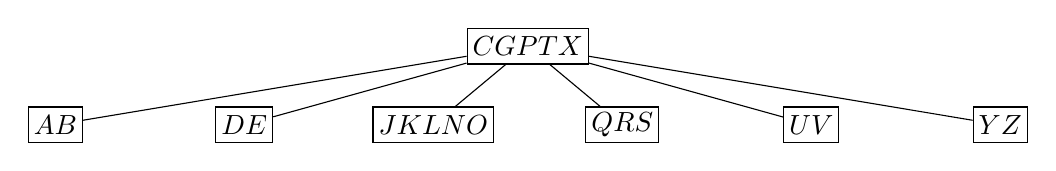
\begin{tikzpicture}[
	level 1/.style={level distance=10mm,sibling distance=24mm},
	level 2/.style={level distance=10mm,sibling distance=16mm},
	level 3/.style={level distance=10mm,sibling distance=16mm},
	inner sep=2pt,every node/.style={draw,rectangle,minimum size=3ex}]
  \node {$CGPTX$}
	child {node {$AB$}}
	child {node {$DE$}}
	child {node {$JKLNO$}}
  	child {node {$QRS$}}
	child {node {$UV$}}
	child {node {$YZ$}}
;
\end{tikzpicture}

\

Recurse.  We are at node $CGPTX$.

``3.  If the key $k$ is not present in internal node $x$, determine the root $x.c_i$ of the appropriate subtree that must contain $k$, if $k$ is in the tree at all.''  The key $B$ must be in the subtree rooted at $x.c_1 = AB$.  

``If $x.c_1$ has only $t-1$ keys, execute step 3a or 3b as necessary to guarantee that we descend to a node containing at least $t$ keys.''  It is true that $x.c_1$ has only $t-1=2$ keys.  

``3a.  If $x.c_i$ has only $t-1$ keys but has an immediate sibling with at least $t$ keys...''  Nope.  

``3b.  If $x.c_i$ and both of $x.c_i$'s immediate siblings have $t-1$ keys, merge $x.c_i$ with one sibling, which involves moving a key from $x$ down into the new merged node to become the median key for that node.''

Merge $AB$ and $DE$, bringing down $C$.  

\

\hfil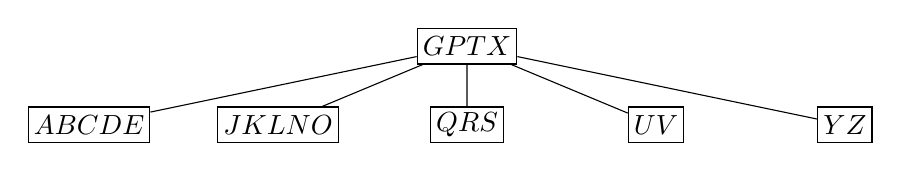
\begin{tikzpicture}[
	level 1/.style={level distance=10mm,sibling distance=24mm},
	level 2/.style={level distance=10mm,sibling distance=16mm},
	level 3/.style={level distance=10mm,sibling distance=16mm},
	inner sep=2pt,every node/.style={draw,rectangle,minimum size=3ex}]
  \node {$GPTX$}
	child {node {$ABCDE$}}
	child {node {$JKLNO$}}
  	child {node {$QRS$}}
	child {node {$UV$}}
	child {node {$YZ$}}
;
\end{tikzpicture}

\

Recurse.  We are at node $x=ABCDE$.  

``1.  If the key $k$ is in node $x$ and $x$ is a leaf, delete the key $k$ from $x$.''  

\

\hfil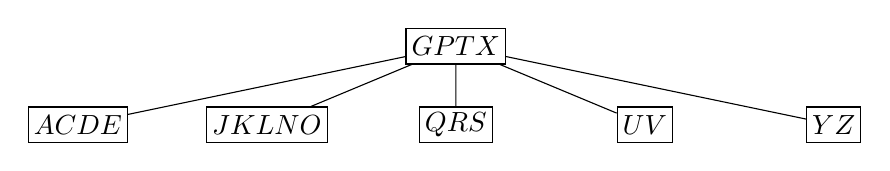
\begin{tikzpicture}[
	level 1/.style={level distance=10mm,sibling distance=24mm},
	level 2/.style={level distance=10mm,sibling distance=16mm},
	level 3/.style={level distance=10mm,sibling distance=16mm},
	inner sep=2pt,every node/.style={draw,rectangle,minimum size=3ex}]
  \node {$GPTX$}
	child {node {$ACDE$}}
	child {node {$JKLNO$}}
  	child {node {$QRS$}}
	child {node {$UV$}}
	child {node {$YZ$}}
;
\end{tikzpicture}

\


{\bf ii.  Insert $M$.}

It's going to go into $JKLNO$, but that would be too big, so split $JKLNO$ into $JK$ and $NO$, moving $L$ up into $GPTX$.  Then insert $M$ into $NO$.  

\

\hfil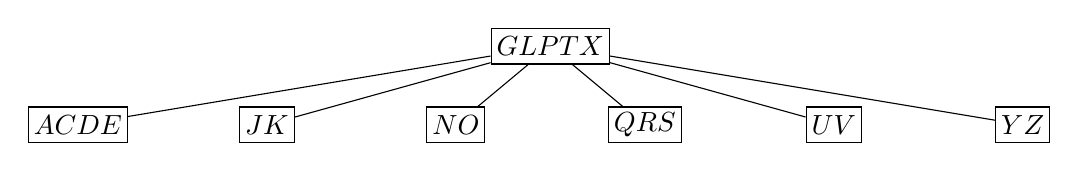
\begin{tikzpicture}[
	level 1/.style={level distance=10mm,sibling distance=24mm},
	level 2/.style={level distance=10mm,sibling distance=16mm},
	level 3/.style={level distance=10mm,sibling distance=16mm},
	inner sep=2pt,every node/.style={draw,rectangle,minimum size=3ex}]
  \node {$GLPTX$}
	child {node {$ACDE$}}
	child {node {$JK$}}
	child {node {$NO$}}
  	child {node {$QRS$}}
	child {node {$UV$}}
	child {node {$YZ$}}
;
\end{tikzpicture}


\

\hfil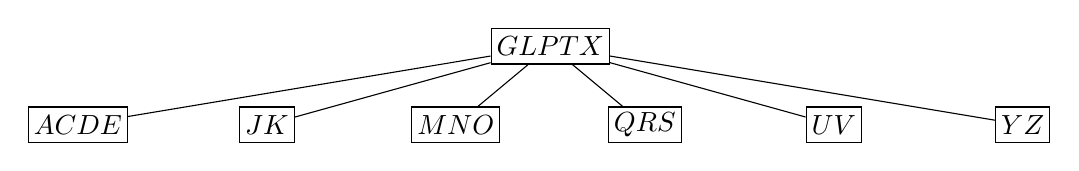
\begin{tikzpicture}[
	level 1/.style={level distance=10mm,sibling distance=24mm},
	level 2/.style={level distance=10mm,sibling distance=16mm},
	level 3/.style={level distance=10mm,sibling distance=16mm},
	inner sep=2pt,every node/.style={draw,rectangle,minimum size=3ex}]
  \node {$GLPTX$}
	child {node {$ACDE$}}
	child {node {$JK$}}
	child {node {$MNO$}}
  	child {node {$QRS$}}
	child {node {$UV$}}
	child {node {$YZ$}}
;
\end{tikzpicture}

\


{\bf iii.  Delete $T$.}  

``2.  If the key $k$ is in node $x$ and $x$ is an internal node, do the following:

a.  If the child $y$ that precedes $k$ in node $x$ has at least $t$ keys, then find the predecessor $k'$ of $k$ in the subtree rooted at $y$.  Recursively delete $k'$, and replace $k$ by $k'$ in $x$.''

In this case, if the key $T$ is in node $GLPTX$ and $GLPTS$ is an internal node, do the following:

a.  If the child $QRS$ that precedes $T$ in node $GLPTX$ has at least $t=3$ keys [which it does], then find the predecessor $S$ of $T$ in the subtree rooted at $QRS$.  Recursively delete $S$, and replace $T$ by $S$ in $GLPTX$.  

\

\hfil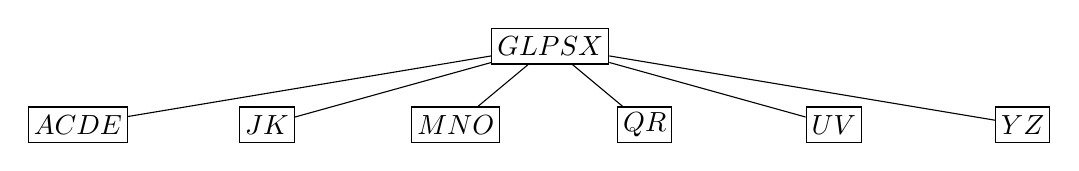
\begin{tikzpicture}[
	level 1/.style={level distance=10mm,sibling distance=24mm},
	level 2/.style={level distance=10mm,sibling distance=16mm},
	level 3/.style={level distance=10mm,sibling distance=16mm},
	inner sep=2pt,every node/.style={draw,rectangle,minimum size=3ex}]
  \node {$GLPSX$}
	child {node {$ACDE$}}
	child {node {$JK$}}
	child {node {$MNO$}}
  	child {node {$QR$}}
	child {node {$UV$}}
	child {node {$YZ$}}
;
\end{tikzpicture}

\



{\bf iv.  Insert $M_t$ for $M < M_t < N$.}  

The first thing to do is to split $GLPSX$.  

\

\hfil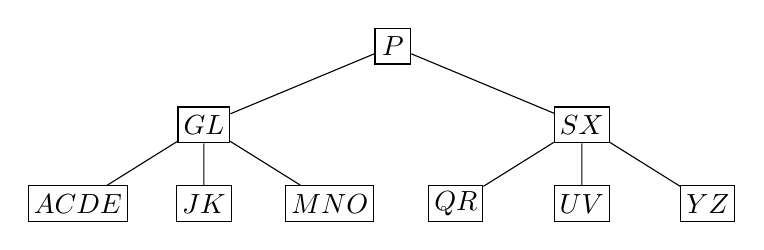
\begin{tikzpicture}[
	level 1/.style={level distance=10mm,sibling distance=48mm},
	level 2/.style={level distance=10mm,sibling distance=16mm},
	level 3/.style={level distance=10mm,sibling distance=16mm},
	inner sep=2pt,every node/.style={draw,rectangle,minimum size=3ex}]
  \node {$P$}
	child {node {$GL$}
		child {node {$ACDE$}}
		child {node {$JK$}}
		child {node {$MNO$}}
	}
  	child {node {$SX$}
	  	child {node {$QR$}}
		child {node {$UV$}}
		child {node {$YZ$}}
	}
;
\end{tikzpicture}

\

Then it's just a leaf insertion.  


\

\hfil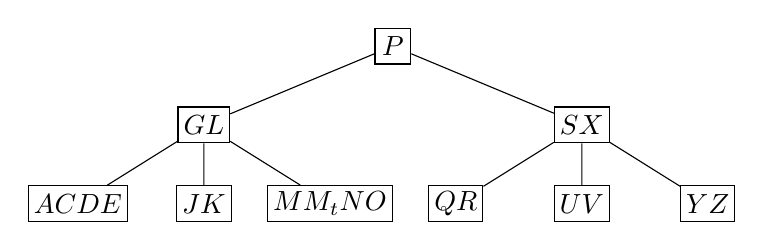
\begin{tikzpicture}[
	level 1/.style={level distance=10mm,sibling distance=48mm},
	level 2/.style={level distance=10mm,sibling distance=16mm},
	level 3/.style={level distance=10mm,sibling distance=16mm},
	inner sep=2pt,every node/.style={draw,rectangle,minimum size=3ex}]
  \node {$P$}
	child {node {$GL$}
		child {node {$ACDE$}}
		child {node {$JK$}}
		child {node {$MM_tNO$}}
	}
  	child {node {$SX$}
	  	child {node {$QR$}}
		child {node {$UV$}}
		child {node {$YZ$}}
	}
;
\end{tikzpicture}

\


%%%%%
\subsubsection{S18 \#L1}
	Given the initial B-tree with the minimum node degree of $t=3$ below, show the results 
	
	\begin{enumerate}[label=\alph*.]
		\item After deleting the key of $M_2$, 
		\item Followed by inserting the key of $L$, 
		\item Then by deleting the key of $J_2$, 
		\item Then by inserting the key of $O_1$ with $O < O_1 < O_2$, and 
		\item Then by deleting $K$.  
	\end{enumerate}
	
	(Show the result after every deletion and after every insertion.)
	
\
	
\hfil	\begin{tikzpicture}[node distance=8 mm and 8 mm]
		\node [rectangle, draw] (a) at (0,0) {$M$};
		\node [rectangle, draw] (b) at (-3,-1) {$J K$};
		\node [rectangle, draw] (c) at (3,-1) {$N O$};
		\node [rectangle, draw, below left=of b] (d) {$A B$};
		\node [rectangle, draw, below=of b] (e) {$J_2 J_3$};
		\node [rectangle, draw, below right=of b] (f) {$K_4 K_6$};
		\node [rectangle, draw, below left=of c] (g) {$M_2 M_4$};
		\node [rectangle, draw, below=of c] (h) {$N_1 N_2 N_3$};
		\node [rectangle, draw, below right=of c] (i) {$O_2 O_3$};
		\foreach \from/\to in {a/b, a/c, b/d, b/e, b/f, c/g, c/h, c/i}
			\draw (\from) -- (\to);
	\end{tikzpicture}
	
	
\subsubsection{Solution}

{\bf Original Tree}

\

\hfil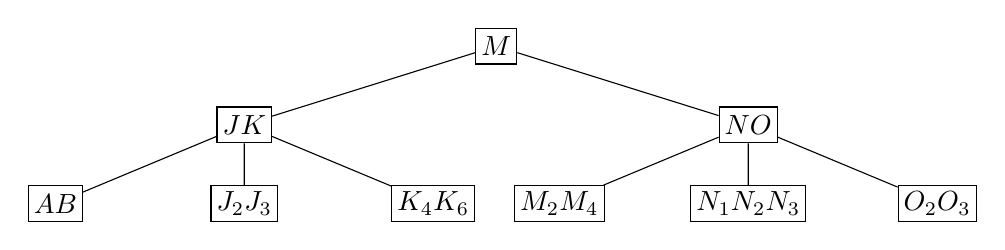
\begin{tikzpicture}[
	level 1/.style={level distance=10mm,sibling distance=64mm},
	level 2/.style={level distance=10mm,sibling distance=24mm},
	level 3/.style={level distance=10mm,sibling distance=16mm},
	inner sep=2pt,every node/.style={draw,rectangle,minimum size=3ex}]
  \node {$M$}
	child {node {$JK$}
		child {node {$AB$}}
		child {node {$J_2 J_3$}}
		child {node {$K_4 K_6$}}
	}
	child {node {$NO$}
		child {node {$M_2 M_4$}}
		child {node {$N_1 N_2 N_3$}}
		child {node {$O_2 O_3$}}
	}
;
\end{tikzpicture}

\

{\bf a. Delete $M_2$.} 

Start on node $M$.  

Instructions on page 502.  

``3.  If the key $k$ [$M_2$] is not present in internal node $x$ [$M$] determine the node $x.c_i$ [$x.c_2 = NO$] of the appropriate subtree that must contain $k$ [$M_2$], if $k$ is in the tree at all.  If $x.c_i$ has only $t-1$ [2] keys, [TRUE], execute step 3a or 3b as necessary to guarantee that we descend to a node containing at least $t$ [3] keys.  Then finish by recursing on the appropriate child of $x$.  

3b.  If $x.c_i$ and both of $x.c_i$'s immediate siblings have $t-1$ [2] keys, merge $x.c_i$ with one sibling, which involves moving a key from $x$ down into the new merged node to become the median key for that node.''  

Consolidate $JK$, $M$, and $NO$.

\

\hfil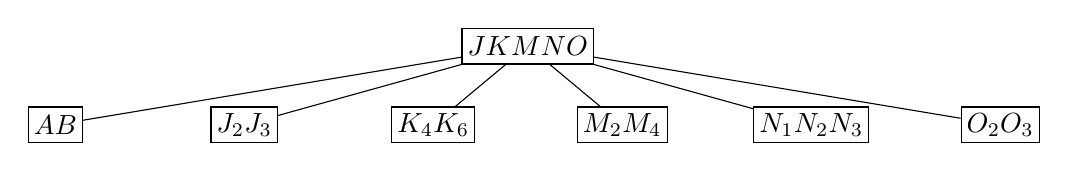
\begin{tikzpicture}[
	level 1/.style={level distance=10mm,sibling distance=24mm},
	level 2/.style={level distance=10mm,sibling distance=24mm},
	level 3/.style={level distance=10mm,sibling distance=16mm},
	inner sep=2pt,every node/.style={draw,rectangle,minimum size=3ex}]
  \node {$JKMNO$}
		child {node {$AB$}}
		child {node {$J_2 J_3$}}
		child {node {$K_4 K_6$}}
		child {node {$M_2M_4$}}
		child {node {$N_1 N_2 N_3$}}
		child {node {$O_2 O_3$}}
;
\end{tikzpicture}

\

``3.  If the key $k$ [$M_2$] is not present in internal node $x$ [$JKMNO$] determine the node $x.c_i$ [$x.c_4 = M_2M_4$] of the appropriate subtree that must contain $k$ [$M_2$], if $k$ is in the tree at all.  If $x.c_i$ has only $t-1$ [2] keys, [TRUE], execute step 3a or 3b as necessary to guarantee that we descend to a node containing at least $t$ [3] keys.  Then finish by recursing on the appropriate child of $x$.  

3a.  If $x.c_i$ [$x.c_4 = M_2M_4$] has only $t-1$ keys but has an immediate sibling with at least $t$ [3] keys, [TRUE], give $x.c_i$ an extra key by moving a key from $x$ [$JKMNO$] down into $x.c_i$, moving a key from $x.c_i$'s immediate left or right sibling up into $x$, and moving the appropriate child pointer [$N$] from the sibling into $x.c_i$.''

Move $N_1$ into $JKMNO$, then move $N$ down into $M_2M_4$.  

\

\hfil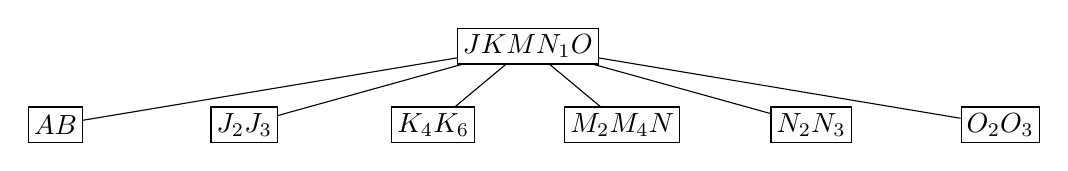
\begin{tikzpicture}[
	level 1/.style={level distance=10mm,sibling distance=24mm},
	level 2/.style={level distance=10mm,sibling distance=24mm},
	level 3/.style={level distance=10mm,sibling distance=16mm},
	inner sep=2pt,every node/.style={draw,rectangle,minimum size=3ex}]
  \node {$JKMN_1O$}
		child {node {$AB$}}
		child {node {$J_2 J_3$}}
		child {node {$K_4 K_6$}}
		child {node {$M_2M_4 N$}}
		child {node {$N_2 N_3$}}
		child {node {$O_2 O_3$}}
;
\end{tikzpicture}

\

Recurse to node $M_2M_4N$.  

``1.  If the key $k$ [$M_2$] is in node $x$ and $x$ is a leaf, [TRUE], delete the node $k$ from $x$.  

\

\hfil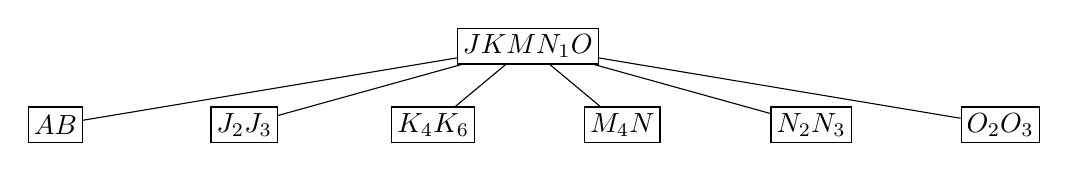
\begin{tikzpicture}[
	level 1/.style={level distance=10mm,sibling distance=24mm},
	level 2/.style={level distance=10mm,sibling distance=24mm},
	level 3/.style={level distance=10mm,sibling distance=16mm},
	inner sep=2pt,every node/.style={draw,rectangle,minimum size=3ex}]
  \node {$JKMN_1O$}
		child {node {$AB$}}
		child {node {$J_2 J_3$}}
		child {node {$K_4 K_6$}}
		child {node {$M_4 N$}}
		child {node {$N_2 N_3$}}
		child {node {$O_2 O_3$}}
;
\end{tikzpicture}

\

{\bf b.  Insert $L$.}  Start by splitting $JKMN_1O$, because it has maximum size and we wouldn't be able to insert something into it if necessary.  

\

\hfil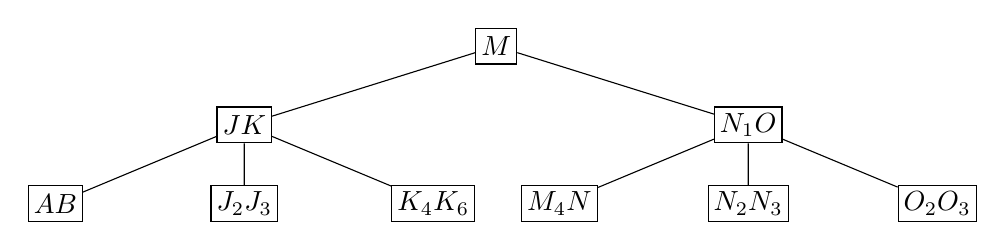
\begin{tikzpicture}[
	level 1/.style={level distance=10mm,sibling distance=64mm},
	level 2/.style={level distance=10mm,sibling distance=24mm},
	level 3/.style={level distance=10mm,sibling distance=16mm},
	inner sep=2pt,every node/.style={draw,rectangle,minimum size=3ex}]
  \node {$M$}
  	child{node{$JK$}
		child {node {$AB$}}
		child {node {$J_2 J_3$}}
		child {node {$K_4 K_6$}}
	}
	child{node{$N_1O$}
		child {node {$M_4 N$}}
		child {node {$N_2 N_3$}}
		child {node {$O_2 O_3$}}
	}
;
\end{tikzpicture}

\

Then it's a leaf insert.  

\

\hfil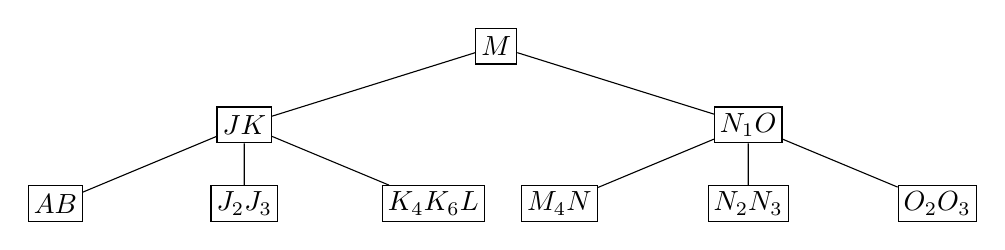
\begin{tikzpicture}[
	level 1/.style={level distance=10mm,sibling distance=64mm},
	level 2/.style={level distance=10mm,sibling distance=24mm},
	level 3/.style={level distance=10mm,sibling distance=16mm},
	inner sep=2pt,every node/.style={draw,rectangle,minimum size=3ex}]
  \node {$M$}
  	child{node{$JK$}
		child {node {$AB$}}
		child {node {$J_2 J_3$}}
		child {node {$K_4 K_6L$}}
	}
	child{node{$N_1O$}
		child {node {$M_4 N$}}
		child {node {$N_2 N_3$}}
		child {node {$O_2 O_3$}}
	}
;
\end{tikzpicture}

\

{\bf c.  Delete $J_2$.}  Re-merge $JK$, $M$, and $N_1O$.  Then rotate $K$ and $K_4$ around to have the minimum number of keys in each node.  

\

\hfil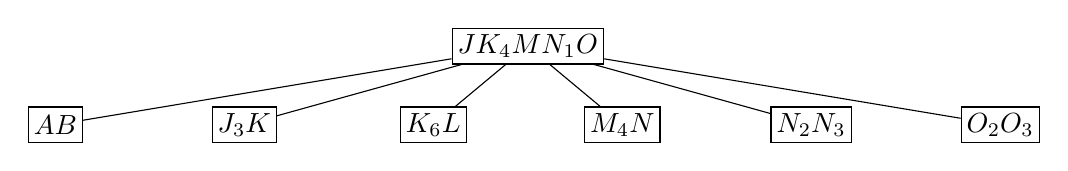
\begin{tikzpicture}[
	level 1/.style={level distance=10mm,sibling distance=24mm},
	level 2/.style={level distance=10mm,sibling distance=24mm},
	level 3/.style={level distance=10mm,sibling distance=16mm},
	inner sep=2pt,every node/.style={draw,rectangle,minimum size=3ex}]
  \node {$JK_4MN_1O$}
		child {node {$AB$}}
		child {node {$J_3 K$}}
		child {node {$K_6 L$}}
		child {node {$M_4 N$}}
		child {node {$N_2 N_3$}}
		child {node {$O_2 O_3$}}
;
\end{tikzpicture}


\

{\bf c.  Insert $O_1$ with $O < O_1 < O_2$.}  Re-split $JK_4MN_1O$, then simple leaf insertion.  

\

\hfil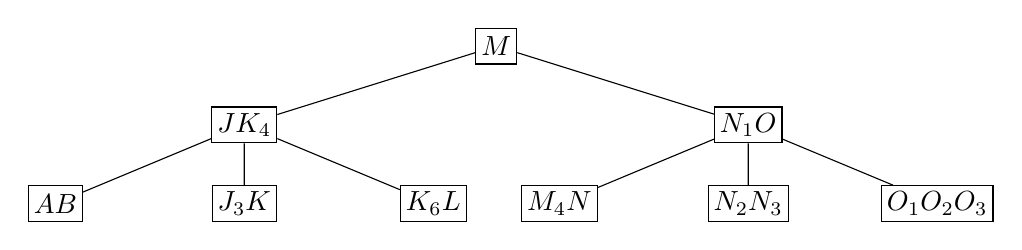
\begin{tikzpicture}[
	level 1/.style={level distance=10mm,sibling distance=64mm},
	level 2/.style={level distance=10mm,sibling distance=24mm},
	level 3/.style={level distance=10mm,sibling distance=16mm},
	inner sep=2pt,every node/.style={draw,rectangle,minimum size=3ex}]
  \node {$M$}
  	child { node{$JK_4$}
		child {node {$AB$}}
		child {node {$J_3 K$}}
		child {node {$K_6 L$}}
	}
	child { node {$N_1O$}
		child {node {$M_4 N$}}
		child {node {$N_2 N_3$}}
		child {node {$O_1 O_2 O_3$}}
	}
;
\end{tikzpicture}


\

{\bf d.  Delete $K$.}  Start with re-merging $JK_4$, $M$, and $N_1O$.    Lots of rotation.  

\

\hfil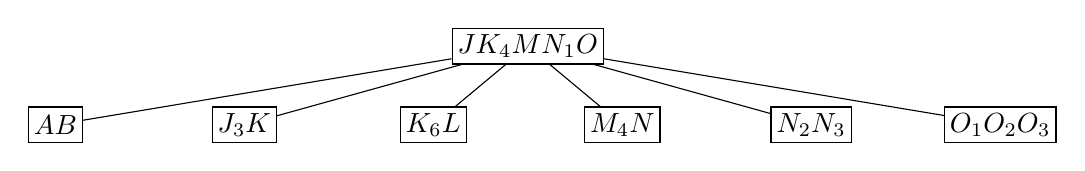
\begin{tikzpicture}[
	level 1/.style={level distance=10mm,sibling distance=24mm},
	level 2/.style={level distance=10mm,sibling distance=24mm},
	level 3/.style={level distance=10mm,sibling distance=16mm},
	inner sep=2pt,every node/.style={draw,rectangle,minimum size=3ex}]
  \node {$JK_4MN_1O$}
		child {node {$AB$}}
		child {node {$J_3 K$}}
		child {node {$K_6 L$}}
		child {node {$M_4 N$}}
		child {node {$N_2 N_3$}}
		child {node {$O_1 O_2 O_3$}}
;
\end{tikzpicture}


\

Rotate  $O$ and $O_1$ left.  

\

\hfil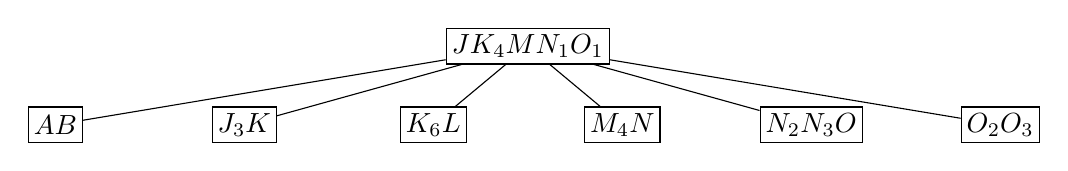
\begin{tikzpicture}[
	level 1/.style={level distance=10mm,sibling distance=24mm},
	level 2/.style={level distance=10mm,sibling distance=24mm},
	level 3/.style={level distance=10mm,sibling distance=16mm},
	inner sep=2pt,every node/.style={draw,rectangle,minimum size=3ex}]
  \node {$JK_4MN_1O_1$}
		child {node {$AB$}}
		child {node {$J_3 K$}}
		child {node {$K_6 L$}}
		child {node {$M_4 N$}}
		child {node {$N_2 N_3O$}}
		child {node {$O_2 O_3$}}
;
\end{tikzpicture}


\

Rotate $N1$ and $N_2$ left.  

\

\hfil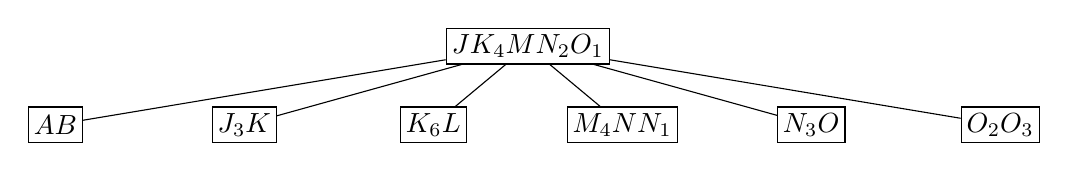
\begin{tikzpicture}[
	level 1/.style={level distance=10mm,sibling distance=24mm},
	level 2/.style={level distance=10mm,sibling distance=24mm},
	level 3/.style={level distance=10mm,sibling distance=16mm},
	inner sep=2pt,every node/.style={draw,rectangle,minimum size=3ex}]
  \node {$JK_4MN_2O_1$}
		child {node {$AB$}}
		child {node {$J_3 K$}}
		child {node {$K_6 L$}}
		child {node {$M_4 N N_1$}}
		child {node {$ N_3O$}}
		child {node {$O_2 O_3$}}
;
\end{tikzpicture}


\

Rotate $M$ and $M_4$ left.  

\

\hfil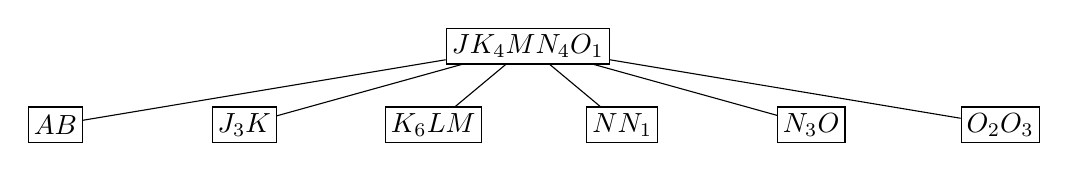
\begin{tikzpicture}[
	level 1/.style={level distance=10mm,sibling distance=24mm},
	level 2/.style={level distance=10mm,sibling distance=24mm},
	level 3/.style={level distance=10mm,sibling distance=16mm},
	inner sep=2pt,every node/.style={draw,rectangle,minimum size=3ex}]
  \node {$JK_4MN_4O_1$}
		child {node {$AB$}}
		child {node {$J_3 K$}}
		child {node {$K_6 L M$}}
		child {node {$N N_1$}}
		child {node {$ N_3O$}}
		child {node {$O_2 O_3$}}
;
\end{tikzpicture}


\

Rotate $K_4$ and $K_6$ left.  

\

\hfil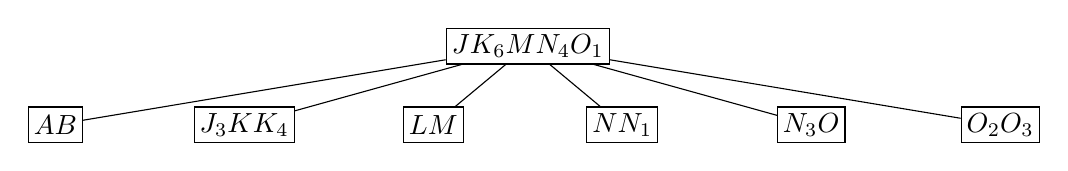
\begin{tikzpicture}[
	level 1/.style={level distance=10mm,sibling distance=24mm},
	level 2/.style={level distance=10mm,sibling distance=24mm},
	level 3/.style={level distance=10mm,sibling distance=16mm},
	inner sep=2pt,every node/.style={draw,rectangle,minimum size=3ex}]
  \node {$JK_6MN_4O_1$}
		child {node {$AB$}}
		child {node {$J_3 K K_4$}}
		child {node {$ L M$}}
		child {node {$N N_1$}}
		child {node {$ N_3O$}}
		child {node {$O_2 O_3$}}
;
\end{tikzpicture}


\

Delete $K$ from the node.

\

\hfil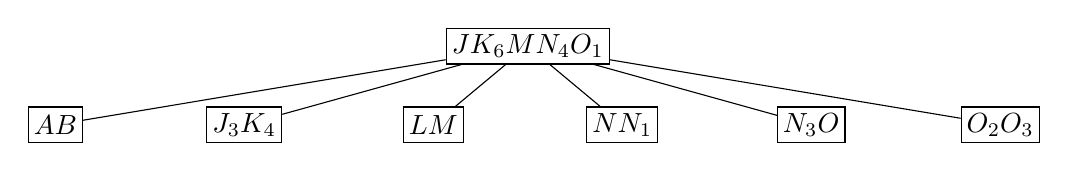
\begin{tikzpicture}[
	level 1/.style={level distance=10mm,sibling distance=24mm},
	level 2/.style={level distance=10mm,sibling distance=24mm},
	level 3/.style={level distance=10mm,sibling distance=16mm},
	inner sep=2pt,every node/.style={draw,rectangle,minimum size=3ex}]
  \node {$JK_6MN_4O_1$}
		child {node {$AB$}}
		child {node {$J_3 K_4$}}
		child {node {$ L M$}}
		child {node {$N N_1$}}
		child {node {$ N_3O$}}
		child {node {$O_2 O_3$}}
;
\end{tikzpicture}


\







%%%%%
\subsubsection{F18 \#L2}
	Given the initial B-tree with the minimum node degree of $t=3$ below, show the results 
	
	\begin{enumerate}[label=\alph*.]
		\item After deleting the key of $K$, 
		\item Followed by inserting the key of $L$, 
		\item Then by deleting the key of $J_2$, 
		\item Then by inserting the key of $N_4$ with $N_3 < N_4 < O$, and 
		\item Then by deleting $K_4$.  
	\end{enumerate}
	
	(Show the result after every deletion and after every insertion.)
	
\
	
\hfil	\begin{tikzpicture}[node distance=8 mm and 8 mm]
		\node [rectangle, draw] (a) at (0,0) {$M$};
		\node [rectangle, draw] (b) at (-3,-1) {$J K$};
		\node [rectangle, draw] (c) at (3,-1) {$N O$};
		\node [rectangle, draw, below left=of b] (d) {$A B$};
		\node [rectangle, draw, below=of b] (e) {$J_2 J_3$};
		\node [rectangle, draw, below right=of b] (f) {$K_4 K_6$};
		\node [rectangle, draw, below left=of c] (g) {$M_2 M_4$};
		\node [rectangle, draw, below=of c] (h) {$N_1 N_2 N_3$};
		\node [rectangle, draw, below right=of c] (i) {$O_2 O_3$};
		\foreach \from/\to in {a/b, a/c, b/d, b/e, b/f, c/g, c/h, c/i}
			\draw (\from) -- (\to);
	\end{tikzpicture}

\

Note:  Same tree as in S18 \#L1, but different keys to insert and delete.  

\subsubsection{Solution}

{\bf Original Tree}

\

\hfil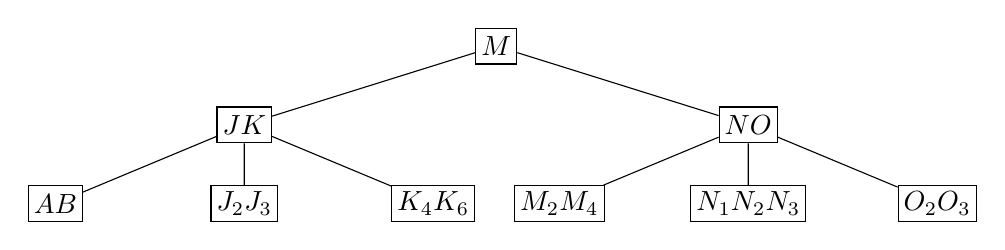
\begin{tikzpicture}[
	level 1/.style={level distance=10mm,sibling distance=64mm},
	level 2/.style={level distance=10mm,sibling distance=24mm},
	level 3/.style={level distance=10mm,sibling distance=16mm},
	inner sep=2pt,every node/.style={draw,rectangle,minimum size=3ex}]
  \node {$M$}
	child {node {$JK$}
		child {node {$AB$}}
		child {node {$J_2 J_3$}}
		child {node {$K_4 K_6$}}
	}
	child {node {$NO$}
		child {node {$M_2 M_4$}}
		child {node {$N_1 N_2 N_3$}}
		child {node {$O_2 O_3$}}
	}
;
\end{tikzpicture}

\

{\bf a.  Delete $K$.}  First, merge $JK$, $M$, and $NO$.  

\

\hfil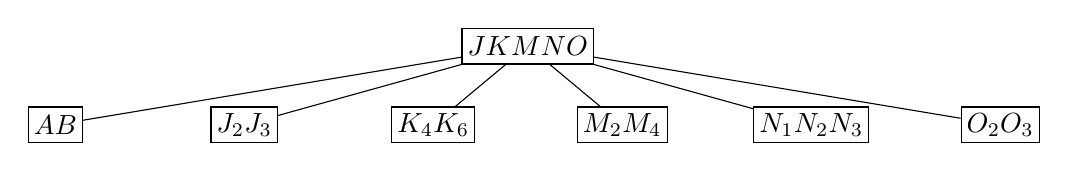
\begin{tikzpicture}[
	level 1/.style={level distance=10mm,sibling distance=24mm},
	level 2/.style={level distance=10mm,sibling distance=24mm},
	level 3/.style={level distance=10mm,sibling distance=16mm},
	inner sep=2pt,every node/.style={draw,rectangle,minimum size=3ex}]
  \node {$JKMNO$}
		child {node {$AB$}}
		child {node {$J_2 J_3$}}
		child {node {$K_4 K_6$}}
		child {node {$M_2M_4$}}
		child {node {$N_1 N_2 N_3$}}
		child {node {$O_2 O_3$}}
;
\end{tikzpicture}

\

Then delete $K$ and merge $J_2 J_3$ and $K_4 K_6$.

\

\hfil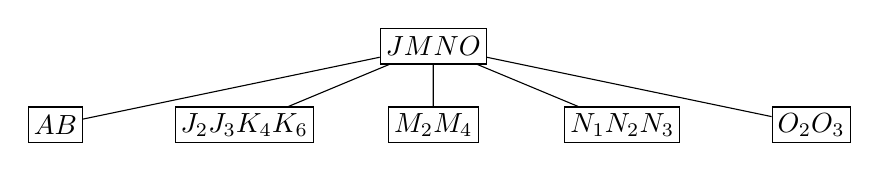
\begin{tikzpicture}[
	level 1/.style={level distance=10mm,sibling distance=24mm},
	level 2/.style={level distance=10mm,sibling distance=24mm},
	level 3/.style={level distance=10mm,sibling distance=16mm},
	inner sep=2pt,every node/.style={draw,rectangle,minimum size=3ex}]
  \node {$JMNO$}
		child {node {$AB$}}
		child {node {$J_2 J_3 K_4 K_6$}}
		child {node {$M_2M_4$}}
		child {node {$N_1 N_2 N_3$}}
		child {node {$O_2 O_3$}}
;
\end{tikzpicture}

\

{\bf b.  Insert $L$.}  Just a simple leaf insert.  

\

\hfil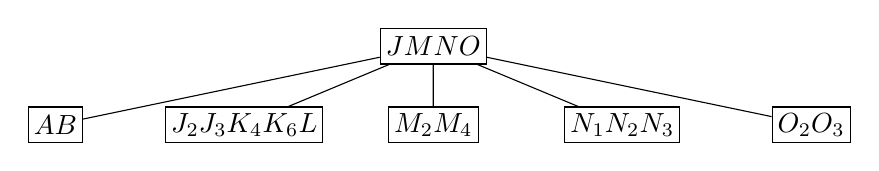
\begin{tikzpicture}[
	level 1/.style={level distance=10mm,sibling distance=24mm},
	level 2/.style={level distance=10mm,sibling distance=24mm},
	level 3/.style={level distance=10mm,sibling distance=16mm},
	inner sep=2pt,every node/.style={draw,rectangle,minimum size=3ex}]
  \node {$JMNO$}
		child {node {$AB$}}
		child {node {$J_2 J_3 K_4 K_6 L$}}
		child {node {$M_2M_4$}}
		child {node {$N_1 N_2 N_3$}}
		child {node {$O_2 O_3$}}
;
\end{tikzpicture}


\

{\bf c.  Delete $J_2$.}  Just a simple leaf deletion.

\

\hfil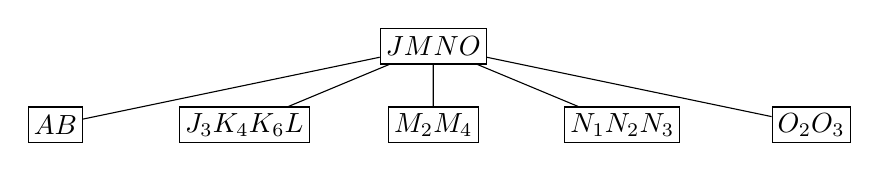
\begin{tikzpicture}[
	level 1/.style={level distance=10mm,sibling distance=24mm},
	level 2/.style={level distance=10mm,sibling distance=24mm},
	level 3/.style={level distance=10mm,sibling distance=16mm},
	inner sep=2pt,every node/.style={draw,rectangle,minimum size=3ex}]
  \node {$JMNO$}
		child {node {$AB$}}
		child {node {$J_3 K_4 K_6 L$}}
		child {node {$M_2M_4$}}
		child {node {$N_1 N_2 N_3$}}
		child {node {$O_2 O_3$}}
;
\end{tikzpicture}

\


{\bf d.  Insert $N_4$ with $N_3 < N_4 < O$.}  Just a simple leaf insertion.

\

\hfil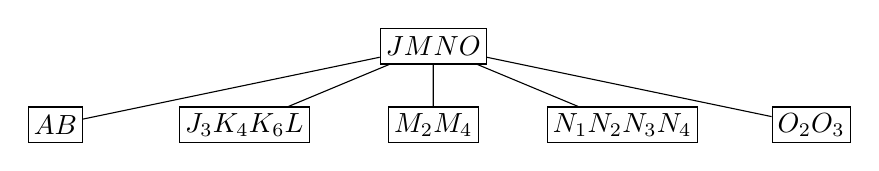
\begin{tikzpicture}[
	level 1/.style={level distance=10mm,sibling distance=24mm},
	level 2/.style={level distance=10mm,sibling distance=24mm},
	level 3/.style={level distance=10mm,sibling distance=16mm},
	inner sep=2pt,every node/.style={draw,rectangle,minimum size=3ex}]
  \node {$JMNO$}
		child {node {$AB$}}
		child {node {$J_3 K_4 K_6 L$}}
		child {node {$M_2M_4$}}
		child {node {$N_1 N_2 N_3 N_4$}}
		child {node {$O_2 O_3$}}
;
\end{tikzpicture}

\


{\bf e.  Delete $K_4$.}  Just a simple leaf deletion.

\

\hfil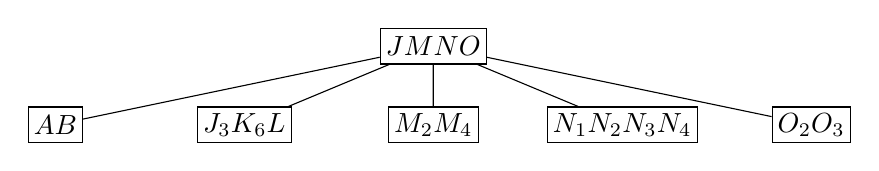
\begin{tikzpicture}[
	level 1/.style={level distance=10mm,sibling distance=24mm},
	level 2/.style={level distance=10mm,sibling distance=24mm},
	level 3/.style={level distance=10mm,sibling distance=16mm},
	inner sep=2pt,every node/.style={draw,rectangle,minimum size=3ex}]
  \node {$JMNO$}
		child {node {$AB$}}
		child {node {$J_3 K_6 L$}}
		child {node {$M_2M_4$}}
		child {node {$N_1 N_2 N_3 N_4$}}
		child {node {$O_2 O_3$}}
;
\end{tikzpicture}

\

%%%%%	
\subsubsection{F16 \#L3}
	Given an initial B-tree with the minimum node degree of $t=2$ below, show the results 
	\begin{enumerate}
		\item after inserting the key of $H$, and 
		\item then followed by deleting two keys in order:  $X$ then $P$.  (show the result after insertion and the result after each deletion.)
	\end{enumerate}
	
\
	
\hfil	\begin{tikzpicture}[x=12mm, y=15mm]
		\node [rectangle, draw] (0) at (0,0) {$P$};
		\node [rectangle, draw] (1) at (-4,-1) {$C G M$};
		\node [rectangle, draw] (2) at (3,-1) {$T X$};
		\node [rectangle, draw] (3) at (-7,-2) {$A B$};
		\node [rectangle, draw] (4) at (-5,-2) {$D E F$};
		\node [rectangle, draw] (5) at (-3,-2) {$J K L$};
		\node [rectangle, draw] (6) at (-1,-2) {$N O$};
		\node [rectangle, draw] (7) at (1,-2) {$Q R S$};
		\node [rectangle, draw] (8) at (3,-2) {$U V$};
		\node [rectangle, draw] (9) at (5,-2) {$Y Z$};
		\draw [-triangle 60] (0) -- (1); 
		\draw [-triangle 60] (0) -- (2); 
		\draw [-triangle 60] (1) -- (3); 
		\draw [-triangle 60] (1) -- (4); 
		\draw [-triangle 60] (1) -- (5); 
		\draw [-triangle 60] (1) -- (6); 
		\draw [-triangle 60] (2) -- (7); 
		\draw [-triangle 60] (2) -- (8); 
		\draw [-triangle 60] (2) -- (9); 
	\end{tikzpicture}
	
\subsubsection{Solution}

{\bf Original Tree}

\	
	
\hfil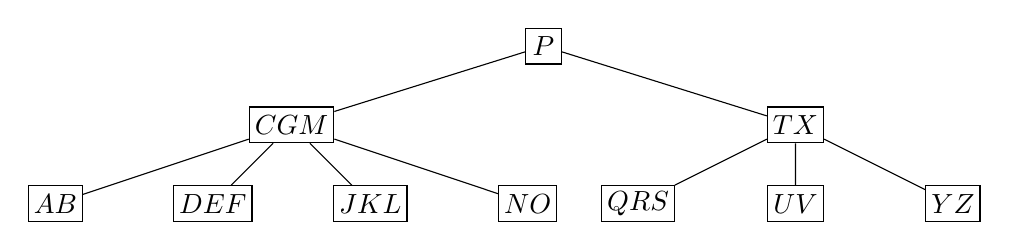
\begin{tikzpicture}[
	level 1/.style={level distance=10mm,sibling distance=64mm},
	level 2/.style={level distance=10mm,sibling distance=20mm},
	level 3/.style={level distance=10mm,sibling distance=16mm},
	inner sep=2pt,every node/.style={draw,rectangle,minimum size=3ex}]
  \node {$P$}
		child {node {$CGM$}
			child {node {$AB$}}
			child {node {$DEF$}}
			child {node {$JKL$}}
			child {node {$NO$}}
		}
		child {node {$TX$}
			child {node {$QRS$}}
			child {node {$UV$}}
			child {node {$YZ$}}
		}
;
\end{tikzpicture}

\

{\bf Insert $H$.}  As we go down the tree toward where $H$ should go, we encounter a full node, $CGM$, so we have to split it.  

\	
	
\hfil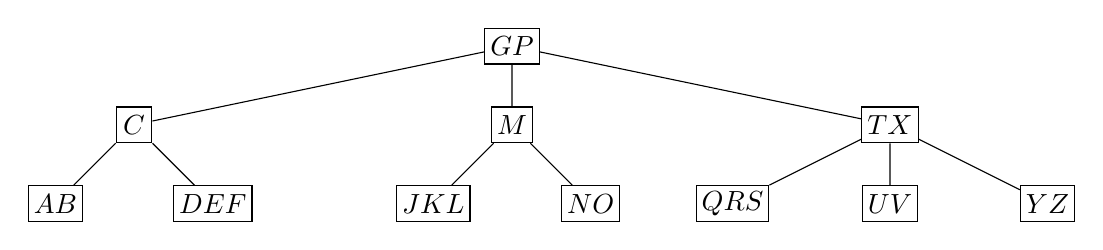
\begin{tikzpicture}[
	level 1/.style={level distance=10mm,sibling distance=48mm},
	level 2/.style={level distance=10mm,sibling distance=20mm},
	level 3/.style={level distance=10mm,sibling distance=16mm},
	inner sep=2pt,every node/.style={draw,rectangle,minimum size=3ex}]
  \node {$GP$}
		child {node {$C$}
			child {node {$AB$}}
			child {node {$DEF$}}
		}
		child {node {$M$}
			child {node {$JKL$}}
			child {node {$NO$}}
		}
		child {node {$TX$}
			child {node {$QRS$}}
			child {node {$UV$}}
			child {node {$YZ$}}
		}
;
\end{tikzpicture}

\

Then going down we want to insert $H$ in $JKL$, but it is full, so we have to split it.  

\	
	
\hfil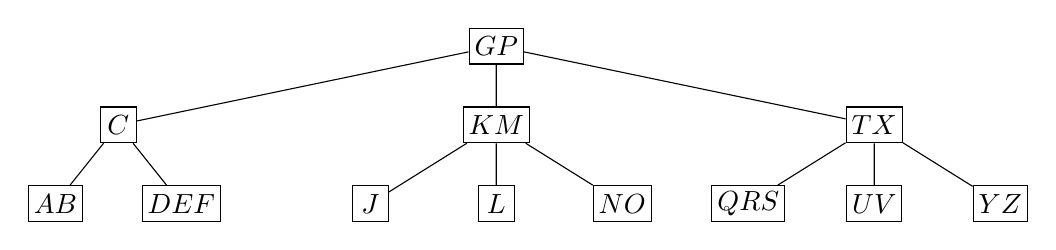
\begin{tikzpicture}[
	level 1/.style={level distance=10mm,sibling distance=48mm},
	level 2/.style={level distance=10mm,sibling distance=16mm},
	level 3/.style={level distance=10mm,sibling distance=16mm},
	inner sep=2pt,every node/.style={draw,rectangle,minimum size=3ex}]
  \node {$GP$}
		child {node {$C$}
			child {node {$AB$}}
			child {node {$DEF$}}
		}
		child {node {$KM$}
			child {node {$J$}}
			child {node {$L$}}
			child {node {$NO$}}
		}
		child {node {$TX$}
			child {node {$QRS$}}
			child {node {$UV$}}
			child {node {$YZ$}}
		}
;
\end{tikzpicture}

\

Now we can insert $H$.  


\	
	
\hfil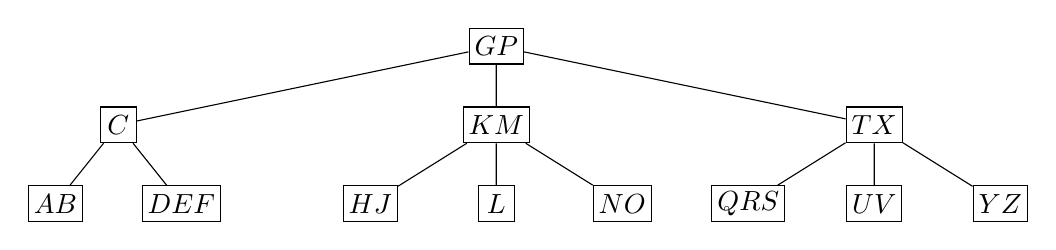
\begin{tikzpicture}[
	level 1/.style={level distance=10mm,sibling distance=48mm},
	level 2/.style={level distance=10mm,sibling distance=16mm},
	level 3/.style={level distance=10mm,sibling distance=16mm},
	inner sep=2pt,every node/.style={draw,rectangle,minimum size=3ex}]
  \node {$GP$}
		child {node {$C$}
			child {node {$AB$}}
			child {node {$DEF$}}
		}
		child {node {$KM$}
			child {node {$HJ$}}
			child {node {$L$}}
			child {node {$NO$}}
		}
		child {node {$TX$}
			child {node {$QRS$}}
			child {node {$UV$}}
			child {node {$YZ$}}
		}
;
\end{tikzpicture}

	
\

{\bf Delete $X$.}  Move $V$ up.  
	


\	
	
\hfil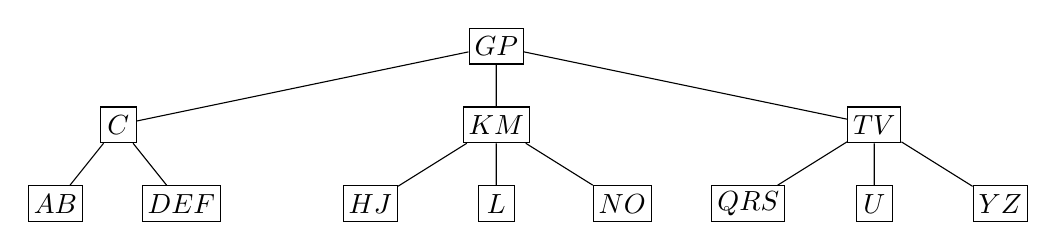
\begin{tikzpicture}[
	level 1/.style={level distance=10mm,sibling distance=48mm},
	level 2/.style={level distance=10mm,sibling distance=16mm},
	level 3/.style={level distance=10mm,sibling distance=16mm},
	inner sep=2pt,every node/.style={draw,rectangle,minimum size=3ex}]
  \node {$GP$}
		child {node {$C$}
			child {node {$AB$}}
			child {node {$DEF$}}
		}
		child {node {$KM$}
			child {node {$HJ$}}
			child {node {$L$}}
			child {node {$NO$}}
		}
		child {node {$TV$}
			child {node {$QRS$}}
			child {node {$U$}}
			child {node {$YZ$}}
		}
;
\end{tikzpicture}

	
\

	
\

{\bf Delete $P$.}  Move $O$ up.  
	


\	
	
\hfil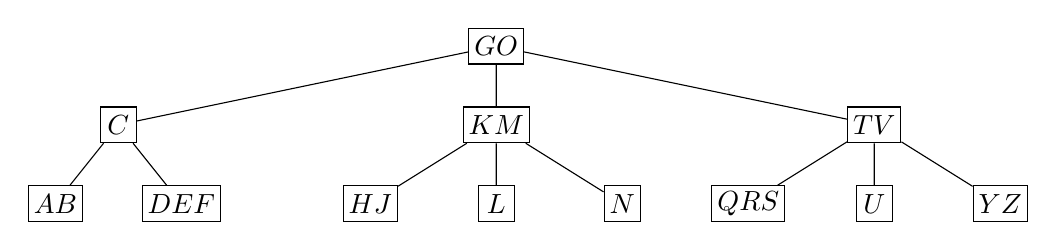
\begin{tikzpicture}[
	level 1/.style={level distance=10mm,sibling distance=48mm},
	level 2/.style={level distance=10mm,sibling distance=16mm},
	level 3/.style={level distance=10mm,sibling distance=16mm},
	inner sep=2pt,every node/.style={draw,rectangle,minimum size=3ex}]
  \node {$GO$}
		child {node {$C$}
			child {node {$AB$}}
			child {node {$DEF$}}
		}
		child {node {$KM$}
			child {node {$HJ$}}
			child {node {$L$}}
			child {node {$N$}}
		}
		child {node {$TV$}
			child {node {$QRS$}}
			child {node {$U$}}
			child {node {$YZ$}}
		}
;
\end{tikzpicture}

	
\

%%%%%
\subsubsection{F15 \#S8}
	For any $n$-key B-tree of height $h$ and with minimum node degree of $t \ge 2$, prove that $h$ is no larger than $\log_t \frac{n+1}{2}$.  (Hint:  Consider the number of keys stored in each tree level.)
	
	

\subsubsection{Solution}	

For illustration, take $t=3$.  In each node is the minimum number of keys in the node.

We're interested in the {\it minimum} number of keys per node, so that we get the maximum possible height for $n$ keys, giving us an upper bound for the height of the tree.  



\


	
\hfil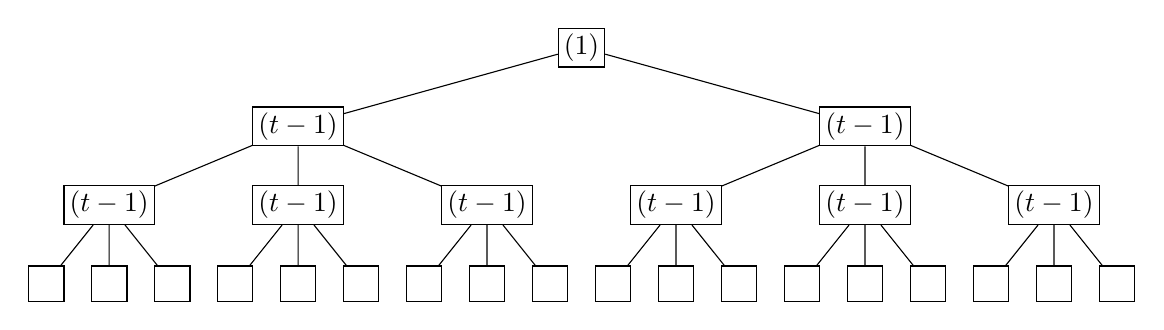
\begin{tikzpicture}[
	level 1/.style={level distance=10mm,sibling distance=72mm},
	level 2/.style={level distance=10mm,sibling distance=24mm},
	level 3/.style={level distance=10mm,sibling distance=8mm},
	inner sep=2pt,every node/.style={draw,rectangle,minimum size=3ex}]
  \node {$(1)$}
		child {node {$(t-1)$}
			child {node {$(t-1)$}
				child {node {}}
				child {node {}}
				child {node {}}
			}
			child {node {$(t-1)$}
				child {node {}}
				child {node {}}
				child {node {}}
			}
			child {node {$(t-1)$}
				child {node {$$}}
				child {node {$$}}
				child {node {$$}}
			}
		}
		child {node {$(t-1)$}
			child {node {$(t-1)$}
				child {node {$$}}
				child {node {$$}}
				child {node {$$}}
			}
			child {node {$(t-1)$}
				child {node {$$}}
				child {node {$$}}
				child {node {$$}}
			}
			child {node {$(t-1)$}
				child {node {$$}}
				child {node {$$}}
				child {node {$$}}
			}
		}
	
;
\end{tikzpicture}

\

The root node (depth 0) has at least one key; thus, two children.  At depth 1, each of the two nodes has at least $t-1$ keys; thus, $t$ children.  At any greater depth, each node has at least $t-1$ keys; thus, $t$ children.  

\

\begin{tabular}{ccc}
	& \multicolumn{2}{c}{Minimum Number of} \cr\cline{2-3}
	Depth & Nodes & Keys \cr\hline
	0 & 1  & 1 \cr
	1 & 2 & $2(t-1)$ \cr
	2 & $2t$ & $2t(t-1)$ \cr
	3 & $2t^2$ & $2t^2(t-1)$ \cr
	& $\vdots$ & \cr
	$h$ & $2t^{h-1}$ & $2t^{h-1}(t-1)$ \cr
\end{tabular}
	
\begin{align*}
	1 + 2(t-1) + 2t(t-1) + 2t^2(t-1) + \cdots + 2t^{h-1}(t-1) &= n \cr
	2(t-1)(1 + t + t^2 + \cdots + t^{h-1}) &= n-1 \cr
	(t-1)\left( \frac{t^h - 1}{t-1} \right) &= \frac{n-1}{2} \cr
	t^h - 1 &= \frac{n-1}{2} \cr
	t^h &= \frac{n-1}{2} + 1 \cr
	t^h &= \frac{n+1}{2} \cr
	 h &= \log_t \frac{n+1}{2} \cr
\end{align*}

\subsubsection{Related Question}

For any $n$-key B-tree of height $h$ and with minimum node degree of $t\ge 2$, find the minimum value of $h$, the height of the tree.  

\

\begin{tabular}{*3{>{$}c<{$}}}
	& \multicolumn{2}{c}{Maximum Number of} \cr\cline{2-3}
	\text{Depth} & \text{Nodes} & \text{Keys} \cr\hline
	0 & 1 & 2t-1 \cr
	1 & 2t & 2t(2t-1) \cr
	2 & (2t)^2 & (2t)^2(2t-1) \cr
	& \vdots \cr
	h & (2t)^h & (2t)^h(2t-1) \cr
\end{tabular}
	
\begin{align*} 
	(2t-1) + 2t(2t-1) + (2t)^2(2t-1) + \cdots (2t)^h(2t-1) &= n \cr
	(2t-1)(1 + (2t) + (2t)^2 + (2t)^h) &= n \cr
	(2t-1)\left( \frac{(2t)^{h+1} - 1}{2t-1} \right) &= n \cr
	(2t)^{h+1} - 1 &= n \cr
	(2t)^{h+1} &= n+1 \cr
	h+1 &= \log_{2t} (n+1) \cr
	h &= \log_{2t}(n+1) - 1 \cr
\end{align*}

\

For any $n$-key B-tree of height $h$ and minimum node degree of $t\ge 2$, 

$$\log_{2t}(n+1) - 1 \le h \le \log_t \frac{n+1}{2}$$

For instance, if $t=2$ and $n=63$, then the height is between 2 and 5.  

$$\log_{2t}(n+1) - 1  = \log_4 64 = 3, \qquad \log_t\frac{n+1}{2} = \log_2 32 = 5$$

%%%%%	
\subsubsection{F15 \#L2}
	Given the initial B-tree with the minimum node degree of $t=3$ below, show the results (a) after inserting two keys in order:  $Q$ then $W$, and (b) followed by deleting two keys in order:  $Y$ then $T$.  (Show the aggregate result after insertion and another result after deletion.)
	
	\
	
\hfil	\begin{tikzpicture}[x=15mm, y=15mm]
		\node [rectangle, draw] (GMPX) at (0,0) {$G \ M \ P \ X$};
		\node [rectangle, draw] (ACDE) at (-4,-1) {$A \ C \ D \ E$};
		\node [rectangle, draw] (JK) at (-2,-1) {$J \ K$};
		\node [rectangle, draw] (NO) at (0,-1) {$N \ O$};
		\node [rectangle, draw] (RSTUV) at (2,-1) {$R \ S \ T \ U \ V$};
		\node [rectangle, draw] (YZ) at (4,-1) {$Y \ Z$};
		\foreach \from/\to in {GMPX/ACDE, GMPX/JK, GMPX/NO, GMPX/RSTUV, GMPX/YZ}
			\draw [-triangle 60] (\from) -- (\to);
	\end{tikzpicture}
	
\subsubsection{Solution}
 
\hfil 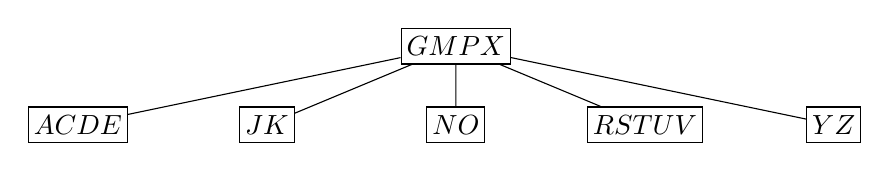
\begin{tikzpicture}[
	level 1/.style={level distance=10mm,sibling distance=24mm},
	level 2/.style={level distance=10mm,sibling distance=24mm},
	level 3/.style={level distance=10mm,sibling distance=8mm},
	inner sep=2pt,every node/.style={draw,rectangle,minimum size=3ex}]
	\node {$GMPX$}
  		child {node {$ACDE$}}
  		child {node {$JK$}}
  		child {node {$NO$}}
  		child {node {$RSTUV$}}
  		child {node {$YZ$}}
	;
\end{tikzpicture}

\	
	
To insert $Q$, we note that $RSTUV$ is full, because $x.n = 5 = 2t-1$, so we must split it by moving $T$ up.  	

\
	
\hfil 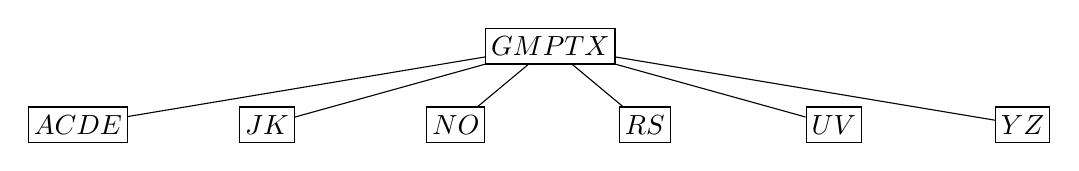
\begin{tikzpicture}[
	level 1/.style={level distance=10mm,sibling distance=24mm},
	level 2/.style={level distance=10mm,sibling distance=24mm},
	level 3/.style={level distance=10mm,sibling distance=8mm},
	inner sep=2pt,every node/.style={draw,rectangle,minimum size=3ex}]
	\node {$GMPTX$}
  		child {node {$ACDE$}}
  		child {node {$JK$}}
  		child {node {$NO$}}
  		child {node {$RS$}}
  		child {node {$UV$}}
  		child {node {$YZ$}}
	;
\end{tikzpicture}	

\
	
Then insert $Q$ into a leaf, simple leaf insertion.  	


\
	
\hfil 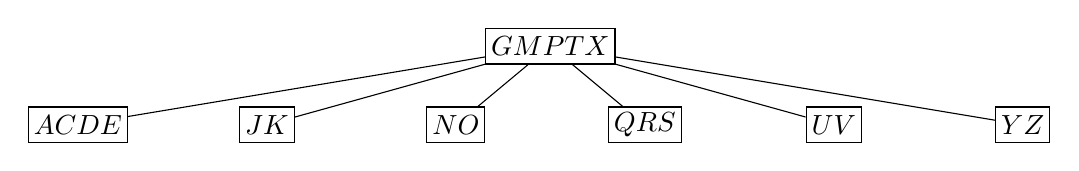
\begin{tikzpicture}[
	level 1/.style={level distance=10mm,sibling distance=24mm},
	level 2/.style={level distance=10mm,sibling distance=24mm},
	level 3/.style={level distance=10mm,sibling distance=8mm},
	inner sep=2pt,every node/.style={draw,rectangle,minimum size=3ex}]
	\node {$GMPTX$}
  		child {node {$ACDE$}}
  		child {node {$JK$}}
  		child {node {$NO$}}
  		child {node {$QRS$}}
  		child {node {$UV$}}
  		child {node {$YZ$}}
	;
\end{tikzpicture}	
	
\

When we go to make another insertion, we hit a full node, $GMPSX$, so we must split it first.  
	

\
	
\hfil 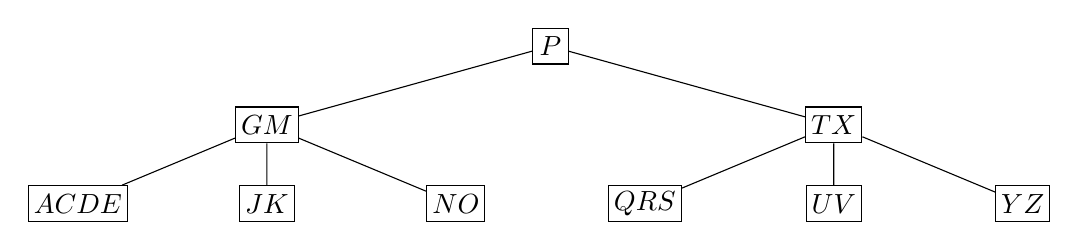
\begin{tikzpicture}[
	level 1/.style={level distance=10mm,sibling distance=72mm},
	level 2/.style={level distance=10mm,sibling distance=24mm},
	level 3/.style={level distance=10mm,sibling distance=8mm},
	inner sep=2pt,every node/.style={draw,rectangle,minimum size=3ex}]
	\node {$P$}
		child {node {$GM$}
	  		child {node {$ACDE$}}
	  		child {node {$JK$}}
	  		child {node {$NO$}}
		}
		child {node {$TX$}
	  		child {node {$QRS$}}
	  		child {node {$UV$}}
	  		child {node {$YZ$}}
		}
	;
\end{tikzpicture}	
	
\

Now $W$ is a simple leaf insertion.  	
	

\
	
\hfil 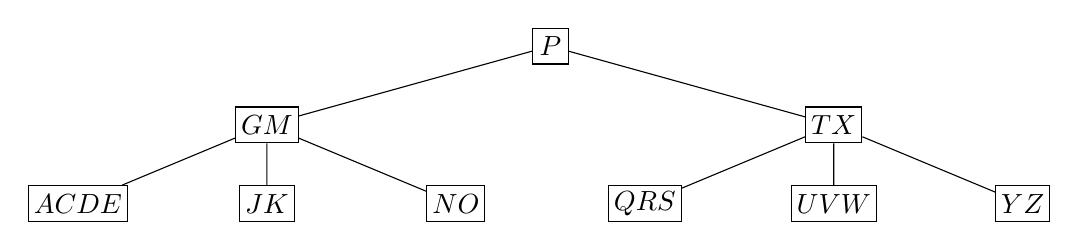
\begin{tikzpicture}[
	level 1/.style={level distance=10mm,sibling distance=72mm},
	level 2/.style={level distance=10mm,sibling distance=24mm},
	level 3/.style={level distance=10mm,sibling distance=8mm},
	inner sep=2pt,every node/.style={draw,rectangle,minimum size=3ex}]
	\node {$P$}
		child {node {$GM$}
	  		child {node {$ACDE$}}
	  		child {node {$JK$}}
	  		child {node {$NO$}}
		}
		child {node {$TX$}
	  		child {node {$QRS$}}
	  		child {node {$UVW$}}
	  		child {node {$YZ$}}
		}
	;
\end{tikzpicture}	
	
\

When we want to delete a key ($Y$), going down the graph we see that we can re-merge $GM$, $P$, and $TX$.  


\
	
\hfil 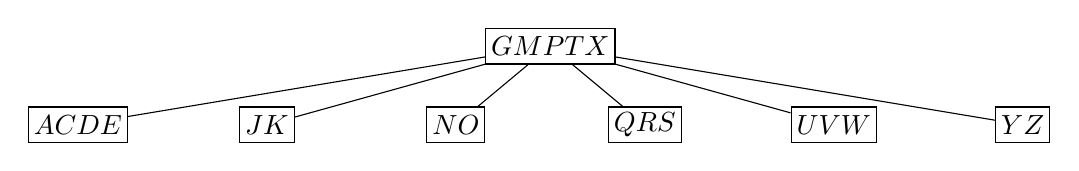
\begin{tikzpicture}[
	level 1/.style={level distance=10mm,sibling distance=24mm},
	level 2/.style={level distance=10mm,sibling distance=24mm},
	level 3/.style={level distance=10mm,sibling distance=8mm},
	inner sep=2pt,every node/.style={draw,rectangle,minimum size=3ex}]
	\node {$GMPTX$}
  		child {node {$ACDE$}}
  		child {node {$JK$}}
  		child {node {$NO$}}
  		child {node {$QRS$}}
  		child {node {$UVW$}}
  		child {node {$YZ$}}
	;
\end{tikzpicture}	
	
\

Now delete $Y$ by rotating $W$ and $X$ around to the right.  	


\
	
\hfil 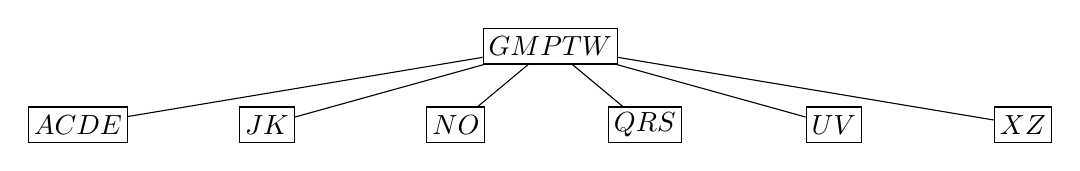
\begin{tikzpicture}[
	level 1/.style={level distance=10mm,sibling distance=24mm},
	level 2/.style={level distance=10mm,sibling distance=24mm},
	level 3/.style={level distance=10mm,sibling distance=8mm},
	inner sep=2pt,every node/.style={draw,rectangle,minimum size=3ex}]
	\node {$GMPTW$}
  		child {node {$ACDE$}}
  		child {node {$JK$}}
  		child {node {$NO$}}
  		child {node {$QRS$}}
  		child {node {$UV$}}
  		child {node {$XZ$}}
	;
\end{tikzpicture}	
	
\

To delete $T$, just merge $QRS$ and $UV$.  

\
	
\hfil 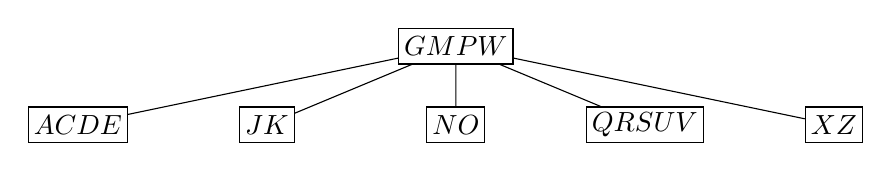
\begin{tikzpicture}[
	level 1/.style={level distance=10mm,sibling distance=24mm},
	level 2/.style={level distance=10mm,sibling distance=24mm},
	level 3/.style={level distance=10mm,sibling distance=8mm},
	inner sep=2pt,every node/.style={draw,rectangle,minimum size=3ex}]
	\node {$GMPW$}
  		child {node {$ACDE$}}
  		child {node {$JK$}}
  		child {node {$NO$}}
  		child {node {$QRSUV$}}
  		child {node {$XZ$}}
	;
\end{tikzpicture}	
	
\

	
	
	
	
	
	

